\documentclass[11pt,a4paper]{article}

% Packages
\usepackage[utf8]{inputenc}
\usepackage[T1]{fontenc}
\usepackage{graphicx}
\usepackage{booktabs}
\usepackage{geometry}
\usepackage{hyperref}
\usepackage{natbib}
\usepackage{amsmath}
\usepackage{xcolor}
\usepackage{float}

% Page layout
\geometry{margin=1in}

% Title information
\title{Technical Analysis Report}
\author{Eduard Ruzga}
\date{\today}

\begin{document}

\maketitle

\begin{abstract}
This document demonstrates a workflow for generating reports that combine technical writing with programmatically generated figures and tables. This template is designed for scientific or technical reports that require data visualization and analysis.
\end{abstract}

\section{Introduction}
\label{sec:introduction}

This document demonstrates an automated workflow for creating technical reports with embedded figures and tables generated from data. It combines the power of \LaTeX{} for document preparation with Python for data processing and visualization.

The workflow consists of:
\begin{itemize}
    \item Python scripts that process data and generate figures
    \item \LaTeX{} document that includes the generated figures
    \item Makefile or shell script that automates the process
\end{itemize}

\section{Time Series Analysis}
\label{sec:timeseries}

Figure \ref{fig:timeseries} shows a comparison between observed temperature data and model predictions over a one-year period. The model generally follows the seasonal pattern, but there are some discrepancies, particularly during extreme temperature events.

\begin{figure}[H]
    \centering
    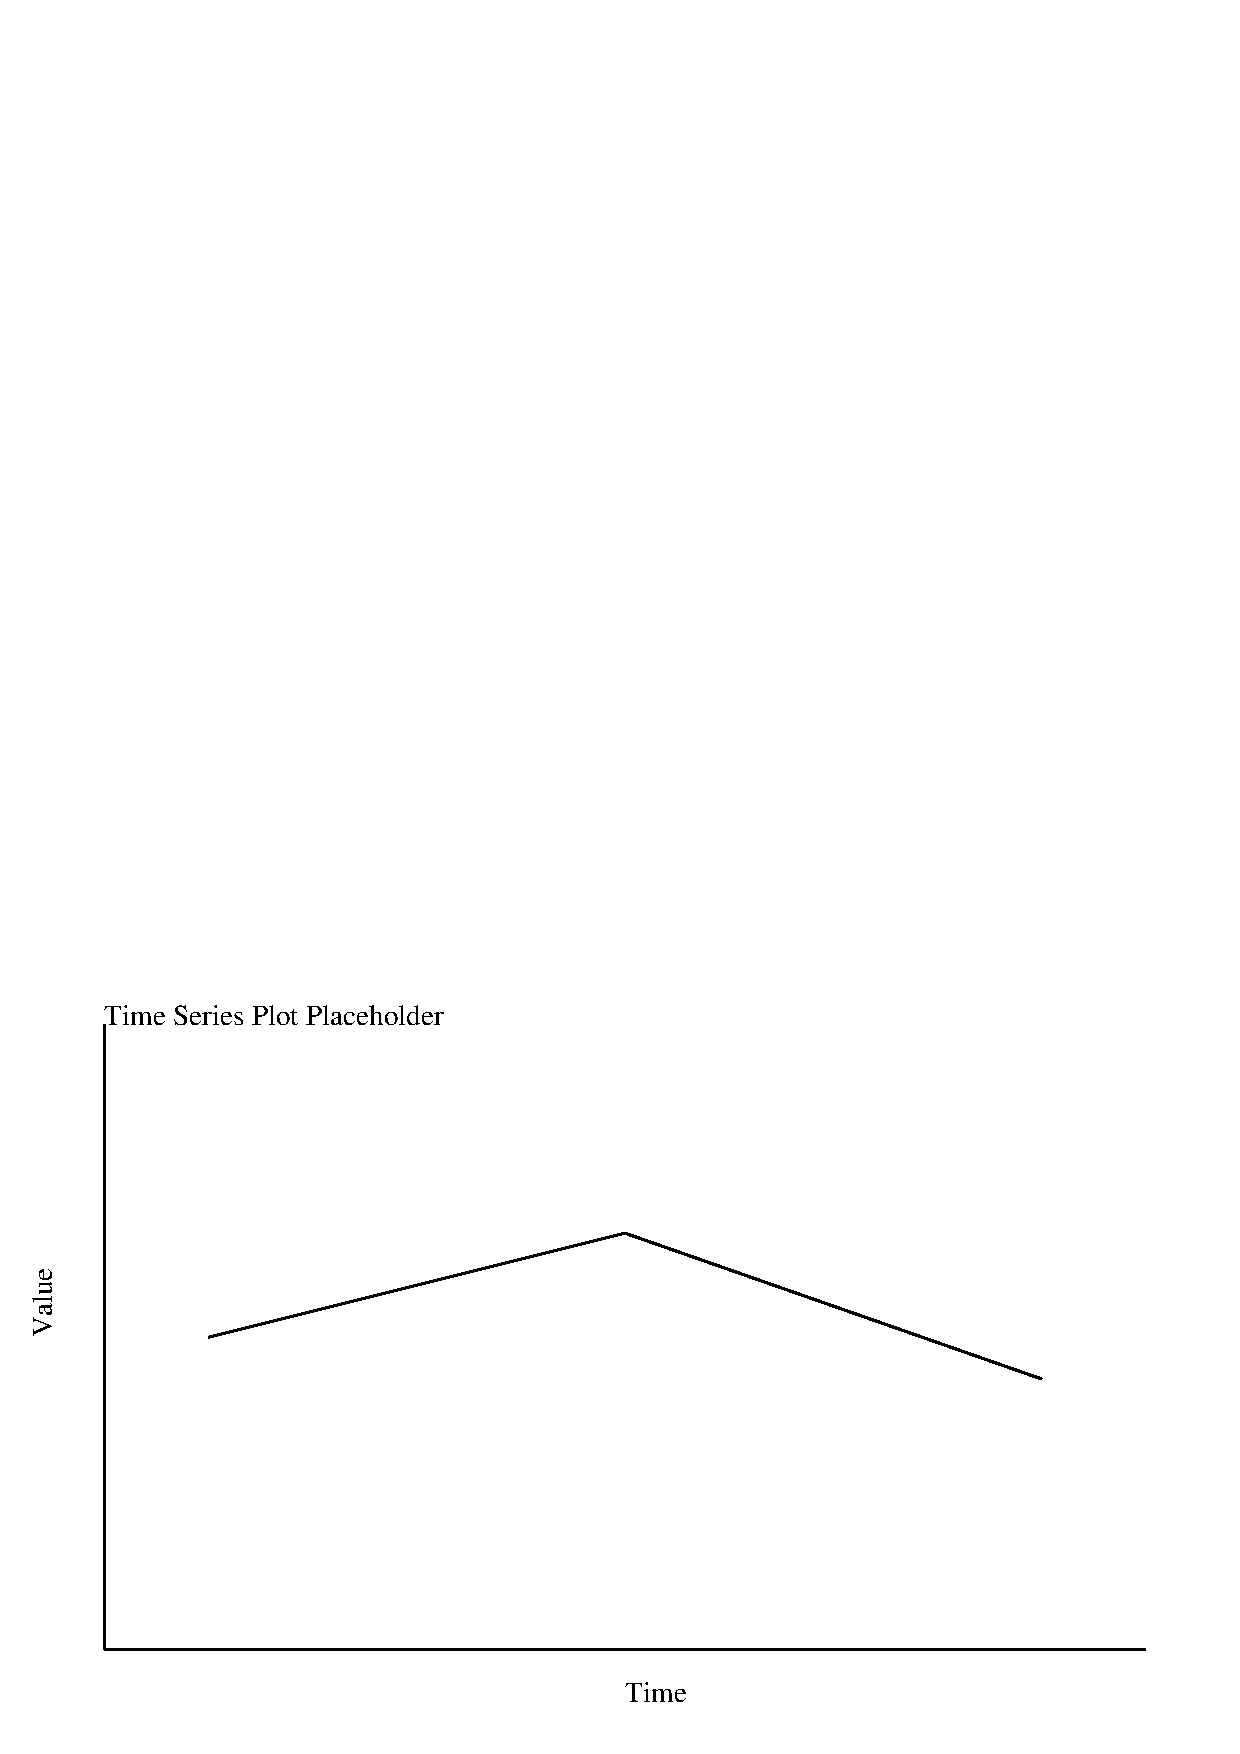
\includegraphics[width=0.8\textwidth]{figures/time_series.pdf}
    \caption{Temperature time series comparison between observations and model predictions.}
    \label{fig:timeseries}
\end{figure}

\section{Spatial Error Analysis}
\label{sec:spatial}

The spatial distribution of errors between observations and model predictions is shown in Figure \ref{fig:errormap}. Areas with positive values indicate where the model underestimates observations, while negative values show overestimation.

\begin{figure}[H]
    \centering
    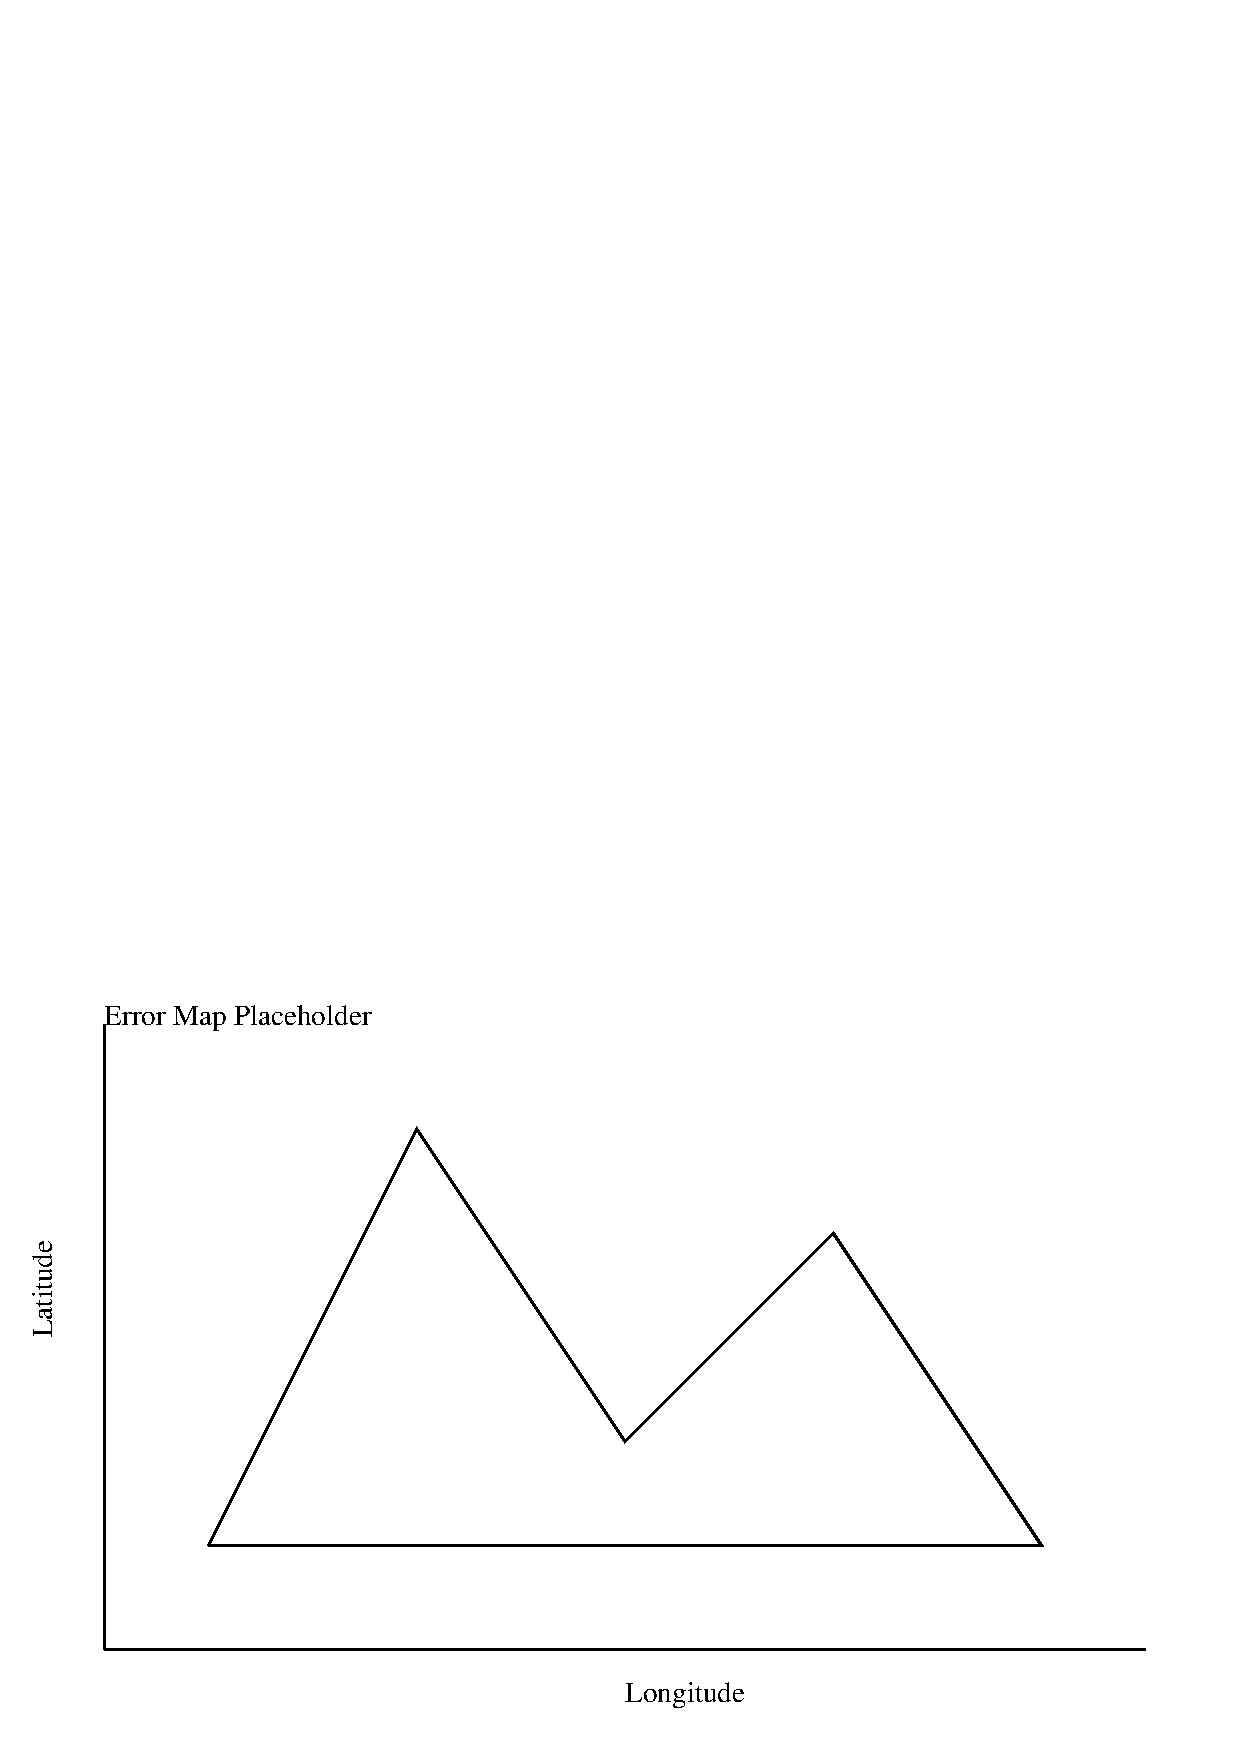
\includegraphics[width=0.7\textwidth]{figures/error_map.pdf}
    \caption{Spatial distribution of errors between observations and model predictions.}
    \label{fig:errormap}
\end{figure}

\section{Regional Performance Statistics}
\label{sec:statistics}

Table \ref{tab:statistics} summarizes the model performance metrics across different regions. The metrics include Root Mean Square Error (RMSE), correlation coefficient, bias, and standard deviation.

\begin{table}[htbp]
\centering
\caption{Statistical Comparison by Region}
\label{tab:statistics}
\begin{tabular}{lrrrr}
\toprule
Region & RMSE & Correlation & Bias & Std Dev \\
\midrule
North & 3.56 & 0.51 & -0.9 & 1.06 \\
South & 3.95 & 0.8 & 1.57 & 0.72 \\
East & 2.69 & 0.51 & -1.13 & 1.76 \\
West & 1.11 & 0.59 & 0.6 & 1.86 \\
Central & 1.88 & 0.77 & 1.24 & 0.52 \\
\bottomrule
\end{tabular}
\end{table}


\section{Conclusion}
\label{sec:conclusion}

This document demonstrated a workflow for generating technical reports with embedded figures and tables. This approach allows for:

\begin{itemize}
    \item Reproducible research and analysis
    \item Consistent formatting and styling
    \item Automated document generation
    \item Version control of both code and document
\end{itemize}

By combining programming for data analysis with \LaTeX{} for document preparation, you can create professional-quality reports efficiently.

\end{document}
